\documentclass[12pt]{amsart}
\setlength{\textwidth}{\paperwidth}
\addtolength{\textwidth}{-2in}
\calclayout

\usepackage{appendix}
\usepackage{tikz}
\usetikzlibrary{automata, positioning}

\newtheorem{theorem}{Theorem}[section]
\newtheorem{corollary}{Corollary}[theorem]
\newtheorem{lemma}[theorem]{Lemma}

\theoremstyle{definition}
\newtheorem{definition}[theorem]{Definition}
\newtheorem{example}[theorem]{Example}
\newtheorem{xca}[theorem]{Exercise}

\theoremstyle{remark}
\newtheorem{remark}[theorem]{Remark}
\numberwithin{equation}{section}

\theoremstyle{remark}
\newtheorem{notation}[theorem]{Notation}

\begin{document}

\title{Annotations on Quantum Pseudorandomness and $k$-Designs}
\author{Edward Kim}
\date{\today}
\maketitle

\begin{abstract}
  We investigate constructions of efficient approximate unitary $k$-designs which are defined as probability distributions over the unitary group which model the Haar distribution up to the $k^{th}$-moment. In particular, we review the paper by Harrow and Low as a directed reading conducted during the Spring 2020 semester.
\end{abstract}

\tableofcontents

\section{Introduction}

The power of randomness in computation is a cornerstone of contemporary computation theory as evidenced by decades of beautiful, celebrated results. Quantum Information has, by no means, become stranger to this trend. Numerous applications of random unitaries have been discovered in the areas of quantum tomography, quantum cryptography, and, rather naturally, quantum algorithms. To gain access to uniformly-sampled elements from $\mathbb{U}(d)$, one must sample from the Haar distribution over $\mathbb{U}(d)$ where $\mathbb{U}(d)$ denotes the group of unitary $d \times d$ matrices. One method of sampling from the Haar distribution is to apply local random unitaries sampled from distributions over lower-dimensional unitary groups. For example, if we consider an $n$-qubit system, one method of sampling from the Haar distribution over $\mathbb{U}(2^n)$ would be through the following scheme:
\begin{enumerate}
  \item Sample from the Haar distribution over $\mathbb{U}(4)$ to produce a random gate $G$
  \item Uniformly pick two distinct qubits and locally apply $G$ to the pair.
\end{enumerate}
However, this becomes computationally infeasible as even reasonably approximating the Haar distribution under this manner requires an exponential number of local 2-qubit gates \cite{knill}. This hurdle motivates us to study the construction of efficient $k$-designs i.e distributions over $\mathbb{U}(4)$ such that sampling over these distributions and applying our scheme above will converge to good approximations of the $k^{th}$ moments of the Haar distributon over $\mathbb{U}(2^n)$. To this end, we begin with annotations of the seminal paper by Harrow and Low \cite{harrlow}. We first introduce concepts germane to the area of efficient $k$-designs and summarize the techniques employed in the analyses presented in the paper.

\section{Approximate 2-designs via Local Random Quantum Circuits}

\subsection{Definitions and Motivations}
In \cite{harrlow}, the authors tackle the problem of approximate $2$-designs, specifically \emph{unitary} $2$-designs. The central result of the paper claims that the scheme of applying sampled $2$-qubit unitaries from certain distributions with a $k$-gapped property converge to the second moment of the Haar distribution rapidly. The crux of the rapid convergence argument relies on mapping the evolution of an initial state under our random circuit to that of a Markov chain's.
Consequently, the analysis becomes amenable to classic techniques created to study mixing times of Markov chains. To begin, we first state the relevant definitions as introduced by Harrow and Low.
%
\begin{remark}
  As dissecting every proof in \cite{harrlow} may unnecessarily length this report, we occasionally omit proofs of lemmas. Some major theorems will have their proofs delegated to the appendix of this report.
\end{remark}

\begin{definition}
  An ensemble of operators $\mathcal{E} = \{p_i, U_i\}$ over $\mathbb{U}(d)$ is called an \emph{(exact) unitary $k$-design} if $\mathcal{G}_W = \mathcal{G}_H$ where
  \begin{align}
    & \mathcal{G}_W(\rho) = \sum_{i} p_i U_i^{\otimes k}\rho (U_i^{\dagger})^{\otimes k} \\
    & \mathcal{G}_H(\rho) = \int_{\mathbb{U}(d)} U^{\otimes k} \rho (U^\dagger)^{\otimes k} \; dU
  \end{align}
\end{definition}
%
 We would naturally like to define some distance between $\mathcal{G}_W$ and $\mathcal{G}_H$. One formulation involves interpreting the two $\mathcal{G}_W, \mathcal{G}_H$ as quantum channels in order to utilize the diamond norm:
%
\begin{definition}
  The diamond norm of an operator $T$ is defined as
  $$||T||_{\diamond} = \sup_d ||T \otimes I_d ||_{\infty} $$
\end{definition}
%
\begin{definition}
  $\mathcal{G}_W$ is an \emph{$\epsilon$-approximate $k$-design} if
  \begin{equation}
    ||\mathcal{G}_W - \mathcal{G}_H ||_{\diamond}  \leq \epsilon
  \end{equation}
\end{definition}
%
As discussed in the introduction above, the unitary constructed by sampling from a universal gate set and applying them to random pairs of qubits will converge to a unitary sampled from Haar distribution. However, we would like to find \emph{efficient approximate} $k$-designs. Here, efficient refers to random circuits of length polynomial in the number of qubits. The authors actually prove some stronger, namely that \emph{$k$-copy gapped} distributions suffice.
%
\begin{definition} \label{gappeddef}
  Let $\mu$ be a (possibly continuous) probability measure on $\mathbb{U}(d)$. If
  \begin{equation}
    \mathcal{G}_{\mu} = \int_{\mathbb{U}(d)} d\mu(U) U^{\otimes k} \otimes (U^*)^{\otimes k}
  \end{equation}
  then we say that $\mathcal{G}_\mu$ is $k$-copy gapped if $\mathcal{G}_\mu$ has only $k!$ unit eigenvalues.
\end{definition}
%
\noindent A more general definition of universality of gatesets can be defined as well:
%
\begin{definition} \label{univdef}
  Let $\mu$ be a distribution over $\mathbb{U}(d)$. $\mu$ is deemed to be \emph{universal} for $\mathbb{U}(d)$ if for any open ball $B \subset \mathbb{U}(d)$, there exists a sufficiently large integer $\ell$ such that $\mu^{\star \ell}(B) > 0$
  where $\mu^{\star \ell}$ refers to the $\ell$-fold \emph{convolution} product of $\mu$:
\end{definition}
%
\begin{equation}
\mu^{\star \ell} = \int_{\mathbb{U}(d)} \delta_{U_1,\cdots, U_\ell} d_\mu(U_1)\cdots d_\mu(U_\ell)
\end{equation}
%
\begin{remark}
  This is the convolution product in the context of \emph{measures}. For example, if we let $\mu,\sigma$ be two finite Borel measures over $\mathbb{R}$, then we have a new finite Borel measure on $\mathbb{R}$, $\mu \star \sigma$:
  $$ \mu \star \sigma(A) = \int_{\mathbb{R}}\int_{\mathbb{R}} \mathbb{I}_A(x+y) d\mu(x)d\sigma(y)$$
  where $\mathbb{I}$ is the characteristic function for measurable set $A \subset \mathbb{R}$.
\end{remark}
\noindent Intuitively, universality implies that sampling enough times over $\mu$ is enough to approximate any gate in $\mathbb{U}(d)$. This aligns with the definition introduced for discrete measures $\mu$ over finite gate sets. We will prove later that any universal gate set will be $k$-copy gapped on $\mathbb{U}(4)$ (Lemma \ref{universal}). For now, let us state the main theorem and its auxiliary lemma to guide our upcoming analysis:
%
\begin{theorem} \label{maintheorem}
  Let $\mu$ be a $2$-copy gapped distribution over $\mathbb{U}(4)$ and $W$ a random circuit of length $t$ drawn from sampling $2$-qubit unitaries from $\mu$ and applying them to random pairs of of a system of $n$-qubits. Then there exists a constant $C$ depending on $\mu$ such that for $\epsilon > 0$, $\mathcal{G}_W$ is an $\epsilon$-approximate $2$-design if $t \geq n(n + \log 1/\epsilon)$.
\end{theorem}
%
\begin{notation}
  Let $\rho$ be an initial state of an $n$-qubit system i.e $\rho \in (\mathbb{C}^{2})^{\otimes n}$. We can expand $\rho$ in terms of the Pauli basis $\{\sigma_i\}_{0 \leq i \leq 3}$ as follows:
  \begin{equation}
    \rho = \frac{1}{2^n} \sum_{p_1,p_2} \gamma_0(p_1,p_2) \sigma_{p_1} \otimes \sigma_{p_2}, \quad \gamma_0(p_1,p_2) \in \in \mathbb{C}
   \end{equation}
  where $p_1,p_2$ run over all strings of Pauli indices of length $n$, $\{0,1,2,3\}^n$. Let $\gamma_W(p_1,p_2)$ be the coefficient of the term $\sigma_{p_1} \otimes \sigma_{p_2}$ for the output state after applying random circuit $W$, $\rho_W = W^{\otimes 2} \rho (W^\dagger)^{\otimes 2}$. Extending this notation allows us to express the expected coefficient after $t$-samples from our distribution $\mu$ as
  $\gamma_t(p_1,p_2) = \mathbb{E}_W [\gamma_W(p_1,p_2)]$. Note that the expectation is taken over all $t$-length random circuits.
\end{notation}

\begin{lemma} \label{mainlemma}
  Let $\rho$ be a an initial state such that $\gamma_0(p,p) \geq 0$ and $\sum_{p} \gamma_0(p,p) = 1$ with $\mu$ and $W$ as in Theorem \ref{maintheorem}. Then there exists constant $C$ such that for $\epsilon > 0$

  \begin{equation}
    \sum_{p_1,p_2 \neq 00} \left( \gamma_t(p_1,p_2) - \delta_{p_1p_2} \frac{1}{2^n(2^n + 1)} \right)^2 \leq \epsilon
  \end{equation}
  for $t \geq Cn\log 1/\epsilon$.

  \begin{equation}
    \sum_{p_1,p_2 \neq 00} \left| \gamma_t(p_1,p_2) - \delta_{p_1p_2} \frac{1}{2^n(2^n + 1)} \right| \leq \epsilon
  \end{equation}
  for $t \geq n(n + \log 1/\epsilon)$
\end{lemma}

\begin{corollary} \label{maincorollary}
  Let $\mu$, $W$, $\gamma_W$ be as above. Then for \emph{any} initial state $\rho$, there exists constant $C$ such that for $\epsilon > 0$,
  \begin{align}
    & \sum_{p_1,p_2 \neq 00} \left( \gamma_t(p_1,p_2) - \delta_{p_1p_2}(\frac{\sum_{p\neq 0} \gamma_0(p,p)}{4^n - 1} \right)^2 \leq \epsilon \\
    & \sum_{p_1,p_2 \neq 00} \left| \gamma_t(p_1,p_2) - \delta_{p_1p_2}(\frac{\sum_{p\neq 0} \gamma_0(p,p)}{4^n - 1} \right| \leq \epsilon
  \end{align}
  both for $t \geq Cn(n + \log 1/ \epsilon)$
\end{corollary}

\subsection{Analysis of Moments}

We turn back to the general case and begin to define concepts and definitions for group $\mathbb{U}(d)$ and for $d$-qudit states. Set a Hermitian basis of $d \times d$ to be $\sigma_0,\sigma_1,\cdots \sigma_{d^2 -1}$ such that $\sigma_0 = I$. These basis elements span the $d$-qudit states. Here we stress that we sample our unitaries over the \emph{Haar distribution} over $\mathbb{U}(d)$. We denote sampling from the Haar distribution with the notation $U \sim \mathbb{U}(d)$ when necessary. Furthermore, our Hermitian basis operators are such that $Tr(\sigma_p\sigma_q) = d \cdot \delta_{p,q}$ i,e orthogonal under the Hilbert-Schmidt inner product. \newline

\noindent Let ${\bf p} = (p_1, \cdots, p_k) \in \{0,1,\cdots, d^2 -1\}^k$ denote a $k$-string of basis indices. We will be interested in the quantity:
%
\begin{equation} \label{Tdef}
  T({\bf p}) := \mathbb{E}_{U \sim \mathbb{U}(d)} \left[ U^{\otimes k} \sigma_{p_1} \otimes \sigma_{p_2} \otimes \cdots \otimes \sigma_{p_k} (U^\dagger)^{\otimes k} \right]
\end{equation}
This will be the expected state after applying a sampled unitary $U$ from the uniform distribution over $\mathbb{U}(d)$. Naturally, we can reexpress this resulting state into the $\sigma_p$ basis:
%
\begin{equation}
  T({\bf p}) = \sum_{{\bf q}} \widehat{G}(\textbf{p},\textbf{q}) \sigma_{q_1} \otimes \cdots \otimes \sigma_{q_k}
\end{equation}
where the same is taken over all $k$-strings in $\{0, \cdots, d^2-1\}^k$. This allows us to define the matrix $\widehat{G}$ where the rows and columns are indiced by $k$-strings with entries $\widehat{G}(\textbf{q},\textbf{p})$. This matrix turns out to be a \emph{symmetric projector}.

\begin{lemma}
  The matrix $\widehat{G}$ above is symmetric i.e. $\widehat{G}(\textbf{p},\textbf{q}) = \widehat{G}(\textbf{q},\textbf{p})$
\end{lemma}
%
\begin{proof}
  By orthogonality:
  \begin{align}
    \widehat{G}(\textbf{q},\textbf{p})
    & = d^{-k} \cdot Tr(\sigma_{q_1} \otimes \cdots \otimes \sigma_{q_k} T(\textbf{p}) ) \\
    & = d^{-k} \mathbb{E}_{U}\left[ Tr(\sigma_{q_1} \otimes \cdots \otimes \sigma_{q_k}) U^{\otimes k} (\sigma_{p_1} \otimes \sigma_{p_2} \otimes \cdots \otimes \sigma_{p_k}) (U^\dagger)^{\otimes k}\right]
  \end{align}
\end{proof}
%
Note that the expectation and the trace operator commute by linearity of latter. The result follows from the cyclic invariance of trace.
%
\begin{lemma} \label{permfix}
$\widehat{G}$ fixes permutation operators $P_{\pi}, \; \pi \in S_k$.
\end{lemma}
%
These two results are all that is required to show that $\widehat{G}$ is indeed a projector.
%
\begin{theorem} \label{g-proj}
  $\widehat{G}$ is a projector i.e. $\widehat{G}^2 = \widehat{G}$
\end{theorem}
%
\begin{proof}
  Expanding the matrix product shows that
  \begin{align}
     \widehat{G}(\textbf{p},\textbf{q})
     & = \sum_{\textbf{q'}} \widehat{G}(\textbf{p},\textbf{q'})\widehat{G}(\textbf{q'},\textbf{q}) = \\
     & = \sum_{\textbf{q'}} \widehat{G}(\textbf{p},\textbf{q'})
          \left( d^{-k} \cdot Tr(\sigma_{q_1'} \otimes \cdots \otimes \sigma_{q_k'}T(\textbf{q})) \right)
  \end{align}
  By Schur-Weyl Duality, $T(\text{q})$ must be a linear combination of permutation operators ($T(\textbf{p})$ commutes with all unitaries of the form $U^{\otimes k}$ by the invariance of the Haar integral). However, by Lemma (\ref{permfix}) above, $\widehat{G}$ fixes the permuatation operators. To understand this more explicitly, rewrite the Lemmma (\ref{permfix}) as follows:
  \begin{equation}
    \sum_{\textbf{q}} \widehat{G}(\textbf{p},\textbf{q})\cdot Tr(\sigma_{q_1} \otimes \cdots \otimes \sigma_{q_k} P_\pi) = Tr(\sigma_{p_1} \otimes \cdots \otimes \sigma_{p_k}P_\pi)
  \end{equation}
  This simply expressing the equality $\widehat{G}P_\pi = P_\pi$ for permutation operator $p_\pi, \; \pi \in S_{k}$. By linearity of trace, the equality above reduces to
  \begin{align}
    \sum_{\textbf{q'}} \widehat{G}(\textbf{p},\textbf{q'})
         \left( d^{-k} \cdot Tr(\sigma_{q_1'} \otimes \cdots \otimes \sigma_{q_k'}T(\textbf{q})) \right)
         & = Tr(\sigma_{p_1} \otimes \cdots \otimes \sigma_{p_k} T(\text{q})) \\
         & = \widehat{G}(\textbf{p},\textbf{q})
  \end{align}
\end{proof}

\begin{corollary}
$\widehat{G}$ has eigenvalues 0 and 1
\end{corollary}

\subsubsection{Explicit calculation of $T(\textbf{p})$} \label{eigenanalysis}
The calculation is divided into the two pertinent cases $k=1,2$. \newline

\begin{enumerate}
  \item \emph{(For $k = 1$)} For this case, a random unitary sampled from the uniform distribution will randomize the initial state. Thus:
  $$
  T(p) = \begin{cases}
    \sigma_0 & p = 0 \\
    0 & p \neq 0
  \end{cases}
  $$
  \item \emph{(For $k=2$)} From Lemma (\ref{permfix}) and Theorem (\ref{g-proj}), $\widehat{G}$ must fix the only two permutation operators $I, \mathcal{F}$ where $\mathcal{F}$ is the swap operator on two qubits. We note that we will normalize the swap operator
  %
  \begin{equation}
    \mathcal{F} = \frac{1}{d^2 -1 }\sum_{1 \leq q \leq d^2 -1} \sigma_{q} \otimes \sigma_{q}
  \end{equation}
  %
  We then deduce the following about $\widehat{G}$: \newline
    \begin{enumerate}
      \item $\widehat{G}(p_1,p_2;q_1,q_2) = 0, \quad p_1 \neq p_2$ or $q_1 \neq q_2$
      \begin{proof}
        To see this, observe that both $I, \mathcal{F}$ have vanishing $\sigma_{q_1} \otimes \sigma_{q_2}$ components for $q_1 \neq q_2$. Thus, multiplying $\widehat{G}$ with either one should also result in vanishing $\sigma_{q_1} \otimes \sigma_{q_2}$ components. This with the fact that all other operators are sent to zero by $\widehat{G}$ yields the result.
      \end{proof}

      \item $\widehat{G}(p;0) = \delta_{p0}$ (Here we denote $\widehat{G}(p;0) := \widehat{G}(p,p;0,0)$)
      \begin{proof}
        This just derives from $\widehat{G}$ acting on $I$
      \end{proof}

      \item $\widehat{G}(p,a) = \frac{1}{d^2-1}, \quad a,p \neq 0$
      \begin{proof}
        As above, this results from $\widehat{G}$ acting on $\mathcal{F}$ along with the condition that it must send all other operators to zero.
      \end{proof}
    \end{enumerate}
    We conclude from the definition of $T(p,q)$ for $p,q \in \{0,\cdots,d^2-1\}$ that
    %
    \begin{equation} \label{concreteT}
      T(p,q) = \begin{cases}
        0 \quad & p \neq q \\
        \sigma_0 \otimes \sigma_0 & p = q = 0 \\
        \frac{1}{d^2 - 1}\sum_{\ell \neq 0}  \sigma_\ell \otimes \sigma_\ell & p = q \neq 0
      \end{cases}
    \end{equation}
\end{enumerate}
%
Recall that $T(p,q)$ refers to the expected \emph{state} from applying unitary $U \sim \mathbb{U}(d)$ to the basis state $\sigma_p \otimes \sigma_q$. From the determination above, it is simple to see that $U$ uniformly samples from all diagonal basis states when acting on $\sigma_p \otimes \sigma_p, \; p \neq 0$. Strikingly enough, applying $U \sim \mathbb{U}(d)$ conserves the total sum of the coefficients of the diagonal basis states.
%
\begin{lemma}
  The total sum of the coefficients $\sum_{p} \gamma_0(p,p)$ is conserved by $U \sim \mathbb{U}(d)$ for state $\rho = \frac{1}{d}\sum_{p_1,p_2} \gamma_0(p_1,p_2) \sigma_{p_1} \otimes \sigma_{p_2}$.
\end{lemma}
%
Normalizing this sum allows us to view it as a \emph{probability distribution}. Furthermore, the evolution of our random circuit scheme is amenable to Markov chain analysis. As an illustrative example, suppose we have an $n$-qubit system and so far have applied $t$ steps of our scheme. As per usual, we pick our $2$-qubit unitary $U \sim \mathbb{U}(4)$. Now if we were to pick qubits $1,2$, our random $2$-qubit unitary would only act on the first two qubits non-trivially whereas every other qubit would just transform via the identity map. By the explicit calculation shown in Equation \ref{concreteT}, the expected \emph{coefficients} for step $t+1$ will work out to be
%
\begin{align} \label{evolexample}
    \gamma_{t+1}(p_1,\cdots,p_n,q_1,\cdots,q_n) = \begin{cases}
       0 & (p_1 ,p_2) \neq (q_1, q_2) \\
       \gamma_t(0,0,\cdots, p_n, 0,0,\cdots,q_n ) & (p_1,p_2) = (q_1, q_2) = (0,0) \\
       \frac{1}{15}\sum_{\substack{r_1,r_2 \\ r_1r_2 \neq 00}} \gamma_t(r_1,r_2,\cdots p_n,r_1,r_2,\cdots,q_n) & (p_1,p_2) = (q_1,q_2) \neq (0,0)
    \end{cases}
\end{align}
 Oliveira et.al \cite{oliveira} had the insight to map the evolution of the $\gamma_t(p,p)$ coeffcients to a Markov chain as follows:
%
\begin{theorem} \label{haarevol}
  Let $M$ be a Markov chain governing the evolution of states under $\widehat{G}$ where $\widehat{G}$ samples from the Haar distribution over $\mathbb{U}(2^n)$. Then $M$ exhibits the following transitions:
  %
  \begin{enumerate}
    \item The states of the Markov chain are $\Omega = \{0,1,2,3\}^n$
    \item The transitions adhere to the guidelines below: Suppose we start with a state indexed by string $\alpha = \alpha_1\cdots\alpha_n$
      \begin{enumerate}
        \item Pick two distinct sites $i < j$ uniformly at random.
        \item If $i = j = 0$, remain at the same state. Otherwise pick $\beta_i\beta_j = \{0,1,2,3\}^2/\{00\}$ uniformly at random. Transition to the string
        $$\alpha_1\alpha_2,\cdots\alpha_{i-1}\beta_i\alpha_{i+1}\cdots \alpha_{j-1}\beta_{j}\alpha_{j+1}\cdots\alpha_n$$
      \end{enumerate}
  \end{enumerate}
\end{theorem}
In the context of the example above, if we start with the coeffcient $\gamma_t(\textbf{q},\textbf{q})$ for $q \in \{0,1,2,3\}^n$, the only two possibilities are $(\textbf{q},\textbf{q}) = (0,0)$ and $(\textbf{q},\textbf{q}) \neq (0,0)$ since it is impossible for the coefficient to vanish by the first case in Equation \ref{evolexample}. Thus, the transitions presented in Theorem \ref{haarevol} indeed lead to the correct expected coefficient value $\gamma_{t+1}(\textbf{p},\textbf{p})$. Note that this is not the complete value for $\gamma_{t+1}$ as we still have to take the expectation over all the remaining qubit pairs.

\subsection{Convergence of the Random Circuit}
Before embarking on the Markov chain analysis, we must prove that our random circuit indeed converges to Haar distribution. This will be proven for the general case of a universal distribution (Definition (\ref{univdef})) on $\mathbb{U}(d)$. Specifcally, we will prove that any universal distribution on $\mathbb{U}(d)$ will be $k$-copy gapped (Definition (\ref{gappeddef})). In turn, this leads to convergence in sense of $\lim_{t \rightarrow \infty} (\widehat{G}_{\mu})^{t} = \widehat{G}_{\mathbb{U}(d)}$. To see this, observe that another formulation of a $k$-copy gapped distributon over $\mathbb{U}(d)$ is
\begin{equation} \label{gappeddis}
  ||G_{\mu} - G_{\mathbb{U}(d)}||_\infty < 1
\end{equation}
where $G_{\mu} = \mathbb{E}_{U \sim \mu} \left[ U^{\otimes k} \otimes (U^\dagger)^{\otimes k} \right]$. To justify this, first recall that $\widehat{G}$ and $G$ are unitarily-related by Definition \ref{Tdef}, so in proving \ref{gappeddis}, we can argue on the operators $\widehat{G}$ instead. In view of this, $\widehat{G}_{\mathbb{U}(d)}$ is a projector and thus has eigenvalues 0 and 1. If we can prove that any eigenvector of $\widehat{G}_{\mathbb{U}(d)}$ of eigenvalue one is also an eigenvector of $\widehat{G}_{\mu}$ of eigenvalue one i.e the $k$-symmetric subspace of $(\mathbb{C}^d)^{\otimes k}$ is also fixed by $\widehat{G}_{\mu}$. Thus, Equation $\ref{gappeddis}$ shows that indeed we can converge to $G_{\mathbb{U}(d)}$ by iterating our scheme (as denoted by $(\widehat{G}_\mu)^t$). Note that $\widehat{G}_{\mu}$ may not even be Hermitian, so we cannot directly argue on its spectrum (as the spectrum may not completely contain real values).
%
\begin{theorem} \label{convergence}
  Let $\mu$ be a universal distribution over $\mathbb{U}(d)$. Then all eigenvectors of $G_{\mathbb{U}(d)}$ of eigenvalue one will also be eigenvectors of $G_{\mu}$ of eigenvalue one. Furthermore, $\mu$ will be $k$-copy gapped.
\end{theorem}
%
\noindent For the sake of presentation, the proof of this will be delegated towards the appendix of this report.
%
\subsection{Markov Chain Analysis}
As discussed in a previous section, the central idea of proving \emph{rapid} convergence involves mapping the evolution of the inital state under our random circuit to that of a Markov chain's. In fact, we can explicitly determine the operator $P$ capturing our dynamics. Let $\widehat{G}^{(ij)}$ denote the unitary transformation resulting from sampling some unitary $U \sim \mathbb{U}(d)$ and applying $U$ to qubits $i$ and $j$ while leaving all other qubits undisturbed.
%
\begin{equation} \label{schemechain}
P = \frac{1}{n(n-1)}\sum_{i \neq j} \widehat{G}^{(ij)}
\end{equation}
as evidenced by the equality
\begin{equation}
  \gamma_{t+1}(\textbf{p}) = \frac{1}{n(n-1)}\sum_{i \neq j}\sum_{\textbf{q}} \widehat{G}^{(ij)}(\textbf{p},\textbf{q})\gamma_t(\textbf{q})
\end{equation}
where $\textbf{p},\textbf{q} \in \{0,1,2,3\}^2$ and $\gamma_t(\textbf{p})$ represents the expected coeffcients at timestep $t$.
%
A major caveat of interpreting $P$ as a \emph{transition matrix} for some suitable Markov chain on the diagonal states $\sigma_p \otimes \sigma_p$ is the possibility that our initial coefficients of diagonal states $\gamma_0(p,p)$ may not even sum to one or even be non-negative. It turns out that this doesn't bring too much trouble into the analysis as pointed out by Corollary \ref{maincorollary}. For now, let us tackle the case where the two conditions above are true and direct our focus on the evolution of the diagonal states. The ultimate goal of this line of thought will be to first prove Lemma \ref{mainlemma} through a carefully-done investigation of the \emph{mixing time} of $P$. Of course, we need to also show that the expected coeffcients of the non-diagonal states $\gamma_0(p,q)$ vanish rapidly as well. These matters will be addressed in a future section.

\subsubsection{Preliminaries on Markov Chains}
Let us introduce some defintions of properties of the Markov chains we are interested in. Although we assume familiarity with the definition of a Markov chain along with the its associated transition matrix $P$, we refer the reader to the reference \cite{cover} for greater detail. Recall that if $q^{(0)}$ is some initial  distribution over the $\Omega$ then $q^{(t)} = q^{(0)}P^t$. The \emph{stationary distribution} of a Markov chain $\pi$ is a probability distribution over $\Omega$ such that $\pi P = \pi$.
%
\begin{definition}
  A Markov chain is said to be \emph{irreducible} if there exists a path $s \rightsquigarrow j$ for every pair of states $s,j \in \Omega$.
\end{definition}
%
\begin{definition}
  A Markov chain is said to be \emph{periodic} at state $i \in \Omega$ if there exists a positive integer $T > 1$ such for that some initial distribution $q^(0)$, if $q_i^{(t)} > 0$ then $t \in \{a + Tm \mid m \in \mathbb{N}\}$. A Markov chain is deemed as \emph{aperiodic} if none of its states are periodic. Equivaently, a Markov chain is aperiodic if all of its states contain self-loops.
\end{definition}
%
\begin{definition}
  A Markov chain is \emph{ergodic} if it is aperiodic and irreducible.
\end{definition}
\noindent As the below theorem reveals, ergodicity shows that any initial distribution over $\Omega$ converges to a unique stationary distribution.
%
\begin{theorem}
  If a Markov chain is ergodic, then it converges to a unique stationary distributon $\pi$ i.e $P$ has a unique eigenvector with eigenvalue one.
\end{theorem}
%
\noindent One can see this through a special case of the \emph{Perron-Frobenius Theorem for Regular Matrices}
%
\begin{theorem} \label{perron}
  Suppose that $P$ is transition matrix with positive entries and also that $P_{ij}^{k} > 0$ for some sufficiently large $k$ and for all entries $i,j$ (Regularity). Then the following must hold:
  \begin{enumerate}
    \item The largest eigenvalue must be real and postive
    \item The largest left eigenvector $\pi$ must be positive and unique
    \item $\lim_{k \rightarrow \infty} qP^{(k)} = \pi$ for all initial distributions $q$.
  \end{enumerate}
\end{theorem}
\noindent Since our matrices are stochastic i.e $\sum_{j} P_{ij} = 1$ for all $i$, our largest eigenvalue will be one. Furthermore, the left eigenvector of eigenvalue one will be the stationary distribution $\pi$. Since our Markov chain is both irreducible and aperiodic, it must be regular as well.
%
\begin{remark}
  It is not difficult to find counterexamples to Theorem \ref{perron} if the Markov chain is not ergodic. For instance, consider the chain

  \begin{figure}[h!]
    \centering
    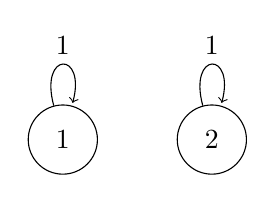
\begin{tikzpicture}
      \node[state]  (one) {1};
      \node[state, right=of one] (two) {2};

      \draw[every loop]
        (one) edge[loop above] node {1} (one)
        (two) edge[loop above] node {1} (two);
    \end{tikzpicture}
    \caption{An aperiodic but reducible chain}
  \end{figure}
  The transition matrix will just be $P = I$. Although the largest eigenvalue is positive and real, its associated left eigenvector is not unique. Thus, it does not have an unique stationary distribution. Another simple chain is

  \begin{figure}[h!]
    \centering
    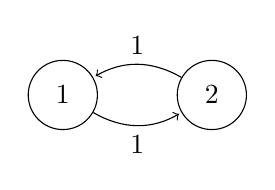
\begin{tikzpicture}
      \node[state]  (one) {1};
      \node[state, right=of one] (two) {2};

      \draw[every loop]
        (one) edge[bend right, auto=right] node {1} (two)
        (two) edge[bend right, auto=right] node {1} (one);
    \end{tikzpicture}
    \caption{An irreducible but periodic chain}
  \end{figure}

  Once again, this chain does not have a unique left eigenvector of unit eigenvalue. Although the stationary distribution $\pi = [\frac{1}{2} \; \frac{1}{2}]$ is unique, no initial distribution converges to it besides $\pi$ itself.

  \begin{figure}[h!]
    \centering
    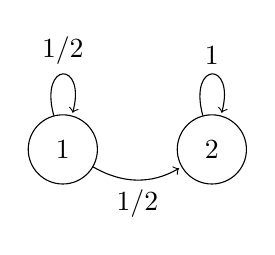
\begin{tikzpicture}
      \node[state]  (one) {1};
      \node[state, right=of one] (two) {2};

      \draw[every loop]
        (one) edge[loop above] node {1/2} (one)
        (one) edge[bend right, auto=right] node {1/2} (two)
        (two) edge[loop above] node {1} (two);
    \end{tikzpicture}
    \caption{An aperiodic, reducible chain which converges}
  \end{figure}
  The transition matrix will be $$ P = \left[ \begin{matrix} \frac{1}{2} & \frac{1}{2} \\
  0 & 1 \end{matrix} \right]$$ which has eigenvalues $\lambda_1 = 1, \lambda_2 = \frac{1}{2}$. Every initial distribution also converges to the unique stationary distribution $\pi = [0 \; 1]$. Hence, this chain exhibits a counterexample to a converse of Theorem \ref{perron}.
\end{remark}
%
%
%Mention counterexamples if time remains
%
\begin{definition}
A Markov chain is \emph{reversible} if the following equality holds for all states $i,j \in \Omega$
\begin{equation}
  \pi(i)P_{ij} = \pi(j)P_{ji}
\end{equation}
\end{definition}
\noindent If the stationary distributon is uniform, then it is simple to see that reversability is equivalent to $P$ being symmetric. Reversability is necessary to invoke certain mixing time lemmas which are introduced in the upcoming section.

\subsubsection{Mixing Times}
We introduce the definition of mixing times presented in \cite{harrlow}. For a deeper treatment of the properties below, see \cite{montenegro}.
%
\begin{definition}
  Let $\pi$ be the stationary distribution of ergodic chain $P$. The 1-norm mixing time $\tau:[0,1] \rightarrow \mathbb{R}$ is real-valued function defined as
  \begin{equation}
    \tau(\epsilon) = \max_q \min_{t \geq 0} ||qP^t - \pi|| \leq \epsilon
  \end{equation}
  where $||p-q|| = \frac{1}{2}\sum_{i \in \Omega} |p_i - q_i|$
\end{definition}
%
\noindent  There is also an associated 2-norm version as well:
%
\begin{definition}
  Let $\pi$ be the stationary distribution of ergodic chain $P$. The 2-norm mixing time $\tau:[0,1] \rightarrow \mathbb{R}$ is real-valued function defined as
  \begin{equation}
    \tau(\epsilon) = \max_q \min_{t \geq 0} ||qP^t - \pi||_2 \leq \epsilon
  \end{equation}
\end{definition}
%
\noindent These definitions allow us to measure the length of time required for a random walk on an ergodic Markov chain to be within $\epsilon$ from the stationary distribution. Consquently, we can express a deep integral inequality bounding the mixing time of an ergodic, reversible chain using its \emph{spectral gap}.
%
\begin{theorem}[Refer to \cite{montenegro}, Corollary 1.15] \label{spectralgap}
  \begin{equation}
    \tau(\epsilon) \leq \frac{1}{\Delta}\log\frac{1}{\pi_*\epsilon}
  \end{equation}
  where $\pi_* = \min_{x \in \Omega} \pi(x)$ and $\Delta = \min{1 - \lambda_2, 1 + \lambda_{min}}$ Here $\lambda_2$ refers to the second largest eigenvalue of $P$ and $\lambda_{min}$ refers to the smallest. This $\Delta$ is known as the spectral gap.
\end{theorem}
\noindent For irreversible chains, the same holds for $PP^*$
%
\begin{theorem}[(Refer to \cite{montenegro}), Corollary 1.14]
  \begin{equation}
    \tau(\epsilon) \leq \frac{2}{\Delta_{PP^*}}\log\frac{1}{\pi_*\epsilon}
  \end{equation}
\end{theorem}
\noindent The inequality can be converted for the 2-norm as well:
%
\begin{equation} \label{2spectralgap}
  \tau_2(\epsilon) \leq \frac{1}{\Delta}\log(1/\epsilon)
\end{equation}

Finally, one more integral tool is required to lower bound the spectral gap of our matrix $P$ in Equation \ref{schemechain}. It is worth stressing that the Markov chain associated to $P_{\mu}$ which we will define as
%
\begin{equation}
P_\mu - \frac{1}{n(n-1)}\sum_{i\neq j}\widehat{G_\mu}^{(ij)}
\end{equation}
For this chain, we sample from a $2$-copy gapped distribution $\mu $ over $\mathbb{U}(4)$ rather than over Haar distribution. It is unclear exactly how this chain evolves as we cannot explicitly compute $P_\mu$ as we did for $P_{\mathbb{U}(d)}$. However, with the \emph{Comparision Theorem}, we can at least lower bound the spectral gap associated with $P_\mu$, say $\Delta_\mu$, with $\Delta_{\mathbb{U}(d)}$. We first state a more general version of the theorem
%
\begin{theorem}[Refer to \cite{montenegro}, Theorem 2.3] \label{comptheorem}
  Let $P$ and $\widehat{P}$ be two Markov chains with the same state space $\Omega$ and the same stationary distribution $\pi$. Then, for ever $x \neq y \in \Omega$ with $\widehat{P}_{xy} > 0$, construct a set of directed paths $\mathcal{P}_{xy}$ from $x$ to $y$ along edges in $P$. Let $\mathcal{P} = \bigsqcup_{x\neq y} \mathcal{P}_{xy}$. We define the flow function $f: \mathcal{P} \rightarrow [0,1]$ such that
  \begin{equation}
    \sum_{\gamma_{xy} \in \mathcal{P}_{xy}} f(\gamma_{xy}) = \widehat{P}_{xy}
  \end{equation}
  then
  $$ \Delta \geq \widehat{\Delta}/A $$
  where
  $$ A = \max_{a \neq b, P_{ab} > 0}\frac{1}{\pi_aP_{ab}} \sum_{x \neq y}\sum_{
                          \substack {
                          \gamma_{xy} \in \mathcal{P}_{xy} \\
                          (a,b) \in \gamma_{xy}}}  \pi(x)f(\gamma_{xy})|\gamma_{xy}|$$
  where $|\gamma_{xy}|$ refers to the length of the path $\gamma_{xy}$.
\end{theorem}
\noindent Note that the bounds yielded will depend on the paths chosen for all $x \neq y \in \Omega$ such that $\widehat{P}_{xy} > 0$ and the values assigned to those paths by the constructed flow function $f$.
\newline

By Theorem \ref{convergence}, both $P_{\mu}$ and $P_{\mathbb{U}(4)}$ converge to same stationary distribution and both share the same state space. Using Theorem \ref{comptheorem}, we can bound the spectral gap of $P_\mu$, $\Delta_\mu$ with the with spectral gap of the $P_{\mathbb{U}(4)}$ chain, $\Delta_{\mathbb{U}(4)}$. However, we must first ensure that the Markov chain associated $P_\mu$ is ergodic. To achieve this, we simply delete the state $\sigma_0 \otimes \sigma_0$ from the state space.   This will turn $P$ into an irreducible chain as $\sigma_0 \otimes \sigma_0$ the only isolated component in the chain. This chain has self-loops by Theorem \ref{haarevol} and thus, it must be ergodic. This puts us in the position to state the lower bound

%Mention Hermitian conjugation at some point.

\begin{theorem} \label{gapbound}
  Let $\mu$ be any 2-copy gapped distribution of gates. If $\mu$ is invariant under Hermitian conjugation then let $\Delta_\mu$ be the spectral gap of resulting Markov chain $P_\mu$. Then
  \begin{equation}
    \Delta_\mu = \Omega(\Delta_{\mathbb{U}(4)})
  \end{equation}
  If $\mu$ is not invariant under Hermitian conjugation, then let $\Delta_{PP^*}$ be the spectral gap of the chain $PP^*$. Then
  \begin{equation}
    \Delta_{PP^*} = \Omega(\Delta_{\mathbb{U}(4)})
  \end{equation}
\end{theorem}
\begin{proof}
  We only show the symmetric case for now. \newline

  First, let us start with an simple example on a 4-qubit system to demonstrate the construction of the relevant paths and flow function. Consider the valid transiton in $P_{\mathbb{U}(4)}$, $1200 \rightsquigarrow 1300$ accomplished by picking sites $1,2$ and transitioning to $1,3$. This shows that $P_{\mathbb{U}(4)}(1200,1300) > 0$. An immediate obstacle arises by observing that this may not a valid transition in the chain $P_\mu$. However, from Section \ref{eigenanalysis}, we know that $\hat{G}_{\mu}$ acts transitively on this subspace of two qubits $\mathbb{C}^4 \otimes \mathbb{C}^4$. Hence, no cycles can exist during the evolution i.e there exists no path $12 \rightsquigarrow \cdots \rightsquigarrow 12$ with length $< 14$. Consequently, only a constant number of transitions have to occur from $12 \rightsquigarrow 13$ and the length of the path cannot be more than $14$. Also, there exists two more possbile transition paths from $1200 \rightsquigarrow 1300$, namely the ones which pick sites $2,3$ and sites $2,4$. The Markov chain just has to transition from $20 \rightsquigarrow 30$ for both cases. This gives us \emph{three} paths from $1200 \rightsquigarrow 1300$ which motivates us to construct our flow function to assign $\frac{1}{3}$ to each path. The procedure for the general case follows similarly: \newline

  We begin by noting that there two cases to consider. Let $h(x,y)$ denote the \emph{Hamming distance} between strings $x,y \in \{0,1,2,3\}^n$ defined to be $h(x,y) = |\{i \in [n] \mid x_i \neq y_i\}|$. There only two cases where $P_{\mathbb{U}(4)}(x,y) > 0$: \newline
  %
  \begin{enumerate}
    \item (\emph{h(x,y) = 2}). Let $i,j$ be the unique indices such that $x_i \neq y_j$. By the discussion above, there exists a constant length path in $P_\mu$, $x \rightsquigarrow y$ acting on sites $i,j$.
    \item (\emph{h(x,y) = 1}). Let $i$ be the index where $x_i \neq y_i$. There are two other subcases in this instance. If the inital state $x_i \neq 0$, then the chain choose any other of the $n-1$ sites to transiton to $y$. To see this, view the desired transition as
    $$x_1 \cdots x_i \cdots x_n \rightsquigarrow y_1 \cdots y_i \cdots y_n$$
    For any $x_j, j < i$ (w.l.o.g), we can transition by $x_jx_i \rightsquigarrow x_jy_i = y_jy_i$. Finally, there is the case when $x_i = 0$. This precludes us from choosing any site containing the identity state $(x_j = 0)$ as $00 \rightsquigarrow 00$ only. This shows us that we can use $n - z(x)$ sites where $z(x)$ denotes the number of zero sites in string $x$.
  \end{enumerate}
  We can now define the flow function $f: \mathcal{P} \rightarrow [0,1]$ through the observations above:
  \begin{enumerate}
    \item (\emph{h(x,y) = 2}) There is only one path $\sigma_{xy}$ in this case. So set $f(\sigma_{xy}) = P_{\mathbb{U}(4)}(x,y) = \Theta(1/n^2)$ by Theorem \ref{haarevol}.
    \item (\emph{h(x,y) = 1}) For the case of non-zero initial value, there are $n-1$ constant-length paths. Equally distributing the weight across all paths shows that $f(\gamma_{xy}) = \frac{P_{\mathbb{U}(4)}(x,y)}{n-1} = \Theta(1/n^2)$ for $\gamma_{xy} \in \mathcal{P}_{xy}$ as $P_{\mathbb{U}(4)}(x,y) = \Theta(1/n)$. For the case of zero initial value: $f(\gamma_{xy}) = \frac{P_{\mathbb{U}(4)}(x,y)}{n-z(x)} = \Theta(1/n^2)$ since ${P_{\mathbb{U}}(4)}(x,y) = \Theta(\frac{n - z(x)}{n^2})$.
  \end{enumerate}
  All that remains is to calculate the number of edges $(a,b)$ such that $P_\mu(a,b) > 0$ and $(a,b) \in \gamma_{xy}$ for some path $\gamma_{xy} \in \mathcal{P}_{xy}$. First, we reduce the expression of the constant $A$ found in Theorem \ref{comptheorem}:
  \begin{align} \label{simplified}
    & A = \max_{a \neq b, \; P_\mu(a,b) > 0} A(a,b) \\
    & A(a,b) = \frac{1}{P(a,b)}\sum_{\substack{\gamma_{xy} \in \sum_{x \neq y}\mathcal{P}_{xy} \\
    (a,b) \in \gamma_{xy}}} f(\gamma_{xy})
  \end{align}
  This arises as $\pi$ is just the uniform distribution and the path lengths $|\gamma_{xy}|$ will always be constant.
  \begin{enumerate}
    \item (\emph{h(a,b) = 2}) Let $i,j$ be the two differing sites. Recall that our paths pick two sites and evolve accordingly. In other words, no path picks two sites and changes sites in the middle of the path (no path evolves like $1200 \rightsquigarrow 1010 \rightsquigarrow 1300$). Furthermore, any such $x,y$ must have $ h(x,y) = 1,2$ in order for it's path $\gamma_{xy}$ to use edge $(a,b)$. There are only a constant number of such pairs $x,y$ which fit the above criterion. Additionally, by the $h(x,y) =2$ case, there is a unique path which \emph{only uses} sites $i,j$ to transition from $x \rightsquigarrow y$. To see this, the case where $h(x,y) = 2$ is simple as there is only one path by construction above. If $h(x,y) = 1$ and (w.l.o.g) only differ at site $i$, then there is only one path from $x$ which picks the exact pair $i,j$ and transitions to $y$. Hence, there are is overall a constant number of paths which can use $(a,b)$. The sum in \ref{simplified} will reduce to $\frac{1}{\Theta(1/n^2)} \cdot \Theta(1/n^2) = \Theta(1)$ as $P_\mu(a,b) = \Theta(1/n^2)$.
    \item (\emph{h(a,b) = 1}) Let $r$ be the number of allowed transitions between $a,b$ (not all pairs may yield direct transitions between $a,b$). We can reduce to the case above for every pair, showing that the sum cumulates to $\Theta(r/n^2)$. As $P_\mu(a,b) = \Theta(r/n^2)$, this once again shows that $A = \Theta(1)$.
  \end{enumerate}
\end{proof}

A significant portion of \cite{harrlow} is dedicated to proving that $\Delta_{\mathbb{U}(4)} = \Theta(1/n)$. Invoking Lemma \ref{spectralgap} and \ref{2spectralgap} along with this tight bound on the spectral gap of the $\mathbb{U}(4)$ chain shows that
%
\begin{corollary} \label{muchainmix}
  The chain $P_\mu$ has 1-norm mixing time $\mathcal{O}(n(n+\log1/\epsilon))$ and 2-norm $\mathcal{O}(n\log\frac{n}{\epsilon})$
\end{corollary}
In fact, by Theorem \ref{gapbound} and Lemma \ref{spectralgap}, the mixing time of the $P_{\mathbb{U}(4)}$ chain upper-bounds the mixing time of the $P_{\mu}$ chain. This mixing time bound is required to finally prove Lemma \ref{mainlemma} as intended.

\subsection{Tight Analysis of $\mathbb{U}(4)$ gap}
In the last section, we used the Comparision Theorem (Theorem \ref{comptheorem}) to bound the gap of the $P_\mu$ chain where $\mu$ is some 2-copy gapped distribution. The rest of this section will be devoted to proving tight bounds on the spectral gap of the $\mathbb{U}(4)$ chain, $\Delta_{\mathbb{U}(4)}$. We reiterate that the Markov chain transitions will be governed as described in Theorem \ref{haarevol}. \newline

For this case, we will just sketch the overarching ideas of the section and leave some details to the appendix of this report and \cite{harrlow}. Once again, we restrict our attention to the coefficients of diagonal states and delete the identity $\sigma_0 \otimes \sigma_0$ in order for the chain to become irreducible. The analysis starts with the consideration of an auxiliary chain called the \emph{zero chain}. The zero chain describes the number of zeros present in a string. The idea is that the number of zeroes slow the mixing process since picking two zeroes effectively changes nothing. If we can show that distribution of zeros mixes well-enough, it can be used to further infer about the mixing of the total chain.
The transition probabilities are worked out in a lemma
%
\begin{lemma} \label{zerochain}
  The zero chain has the following transition matrix $P$ on the state space $\Omega = \{1,2, \cdots,n\}$. This chain actually counts the number of non-zeros of state.
  \begin{equation}
    P(x,y) = \begin{cases}
    1 - \frac{2x(3n-2x -1)}{5n(n-1)} & y = x \\
    \frac{2x(x-1)}{5n(n-1)} & y = x - 1 \\
    \frac{6x(n-x)}{5n(n-1)} & y = x + 1 \\
    0 & \text{otherwise}
    \end{cases}
  \end{equation}
  for $1 \leq x,y \leq n$
\end{lemma}
\begin{proof}
  This can be derived through a simple counting argument. For example, for the number of zeros to decrease ($x$ increases), two sites with a non-zero value and a zero value must be chosen and the chain must transition to pair of non-zero values. $9$ out of the $15$ possible transition values consist of two non-zero values. There the probabilty of picking a zero and a non-zero value is $\frac{2x(n-x)}{n(n-1)}$, bringing the total value to $\frac{9}{15}\frac{2x(n-x)}{n(n-1)} = \frac{6x(n-x)}{5n(n-1)}$.
\end{proof}
% Mention stationary distribution
%
\noindent It is also simple to show that the stationary distribution $\pi_0$ of the zero chain will be
%
\begin{equation}
    \pi_0(x) = \frac{3^x{n \choose x}}{4^n - 1}
\end{equation}
%
The integral property about this zero chain is that it mixes rapidly
%
\begin{theorem} \label{zerochainmixing}
  The zero chain mixes in $\Theta(n\log\frac{n}{\epsilon})$ time.
\end{theorem}
%
\noindent which leads to the rapid mixing of the total chain
\begin{theorem} \label{totalchainmixing}
  The total chain mixes in time $\Theta(n \log\frac{n}{\epsilon})$
\end{theorem}
\begin{remark}
  Diniz and Johnathan point out in \cite{diniz} a faulty assumption made by the authors of \cite{harrlow}. In the proof of Corollary \ref{totalchainmixing},
\end{remark}
The proofs of these two theorems will also be assigned a portion of the appendix.
By the discussion of Corollary \ref{muchainmix}, this proves Lemma \ref{mainlemma}.

%\subsection{Tying Some Loose Ends}


%Finally, we state the proof of Theorem \ref{maintheorem}. \newline
%\begin{proof}[(Proof of Theorem \ref{maintheorem})]
%\end{proof}



\bibliographystyle{amsplain}
\bibliography{biblio}

\end{document}
